\documentclass[12pt]{article}
\usepackage{amsmath}
\usepackage{hyperref}
\usepackage{url}
\usepackage[onehalfspacing]{setspace}
\usepackage[top=2.5cm, bottom=2.5cm, left=2.5cm, right=2.5cm]{geometry}
\usepackage{mathptmx}
\usepackage{enumitem}
\usepackage[style=ieee]{biblatex}
\usepackage{xcolor}
\usepackage{listings}
\usepackage{dirtree}
\usepackage{tabularx}
\usepackage[automake]{glossaries-extra}
\usepackage{graphicx}
\usepackage{float}


\hypersetup{
      colorlinks=true,
}
\setlist{nosep}

\makeglossaries


\newglossaryentry{llvm}
{
    name=LLVM,
    description={LLVM (originally standing for Low Level Virtual Machine) is a system
    of compilers and toolchains and software to create them.}
}

\newglossaryentry{taggedUnion}
{
    name={tagged unions},
    description={Tagged Unions are types whose values can contain several different
    types of which the current type is signified by a value (the tag).}
}

\newabbreviation{ir}{IR}{Intermediate Representation}
\newabbreviation{wasm}{WASM}{Web Assembly}
\newabbreviation{vscode}{VSCode}{Visual Studio Code}
\newabbreviation{gc}{GC}{Garbage Collector}
\newabbreviation{api}{API}{Application Programming Interface}
\newabbreviation{ffi}{FFI}{Foreign Function Interface}

\addbibresource{bibliography.bib}

\title{Creation of a functional programming language\\Maturaarbeit}
\author{Enea Giger\\Betreuungsperson: Adrian Lüthi}
\date{Gymnasium Burgdorf\\\today}

\newcommand{\importListing}[1]{
    \begin{minipage}{\textwidth}
    \input{#1}
    \end{minipage}
}

\begin{document}
\maketitle
\begin{abstract}
	This paper describes the creation of a new functional programming language called Imp
	and both an interpreter and a compiler for it from scratch.
	It describes the essential architecture and algorithms used for those
	implementations including transformation to \Gls{llvm} \gls{ir} and tail call optimization.
	The language itself is aimed to be relatively simple
	and is written almost exclusively in the relatively new language
	Zig.
\end{abstract}
\newpage


\tableofcontents
\newpage

\section{Introduction}
In todays world, computers are omnipresent. Everything depends on them.
And all these computers have to be programmed to do something useful.
Those programs need to be written in some language, which today most
often are imperative languages like C++, JavaScript or Python.
But as recent developments show, parallelism is getting more
and more important. Nowadays, most of the progress in CPUs stems not from
improved performance per core, but from increasing the number of cores included.
Yet in the languages most used to program, parallelism is usually hard to introduce
and requires massive work to introduce because of issues like race conditions.

Functional programming languages solve this problem, because they eliminate side effects
like mutation of variables in a function entirely, which would otherwise prevent functions to be run in
parallel, since the order those side effects happen in, might matter.
This means that programs in functional languages are easier to parallelize and therefore
these languages could become very important in the future.

The removal of side effects is due to functional programming languages being based
on mathematical functions, which give the same result each time, if the input is the same.
This is in contrast to imperative programming languages whose functions are
actually procedures, step by step instructions, that depend on the current state.
Instead of loops, recursion is used in functional languages like in mathematics.
Functional programming languages also have first-class functions, meaning
all functions are values and can therefore be passed around to other functions
or stored in variables.

The main goal of this project was to devise such a functional language
and create an implementation of it.
The principal aim for the syntax of the language was then to keep it simple,
so the focus could lie more on the implementation instead of language design.
To that end it was also the goal to have strict immutability and no loops.
Another aim was to create this implementation with as few dependencies as possible
in order to learn all the basics from scratch and for the language to be fully
cross-platform.

The language was later decided to be called Imp for Impure,
as Input/Output is allowed in this language
without distinguishing functions using it from functions that do not.

\newpage
\section{Fundamentals}
Though programming languages can be very different,
the elementary steps taken in each implementation are
still mostly the same for all languages, no matter the paradigm.

These next paragraphs explain this basic knowledge needed
to understand the structure of this project.

\subsection{The Lexer}
The first step of a programming language implementation is almost always the lexer.
It is responsible for splitting up the source code into tokens,
which are little chunks like the name of a variable or a statement.
These tokens can then be used as input for the parser.

\subsection{The Parser}
The Parser of a programming language is responsible for ensuring the syntax is correct and, in most cases,
building a tree out of the tokens, called Syntax Tree.
This can be done in many ways, though what methods are applicable
depend on the syntax of the language.
\subsubsection{Pratt Parsing}
Pratt Parsing \autocite{prattTopOperatorPrecedence1973}
is one of the most common algorithm for parsing languages.
It works with a list of rules for what to do when a certain type of token is encountered
either at the start or in the middle of an expression.
It works like this:
When parsing an expression using this method,
it starts with the right-binding power of 0.
The right-binding power represents how strong
the preciding operator (if any) binds to the expression
on its right.

Then the first type of token is looked up
in the list of rules for the start
(to get the null denotation, as it is called in the paper).
This lookup results in a function which is then called
which parses the expression starting with this token.
For example, if this is a negation, it also parses the argument
by recursively calling the expression function again with an
appropriate right-binding power.
Once this prefix is parsed the algorithm enters a loop:
\begin{enumerate}
	\item \label{start}
	      Lookup the next token in the in- and postfix table.
	      (This is called the left denotation in the paper.)
	      This results in a left-binding power and a function
	\item If there is no function listed or
	      the left-binding power stored is less or equal
	      to the right-binding power, return the current expression
	      as the operator preceding the current expression binds
	      too strongly, meaning the current operator has a lower precedence.
	      It will be parsed as soon as a call with a low enough
	      right-binding power is reached.
	\item Otherwise, call the parsing function listed with the current expression
	      (its left) and store the result back in the current expression
	\item Return to step \ref{start}.
\end{enumerate}
For infix operators like multiplication, this parsing function
will call the expression function again, but with a higher right-binding power
so as to ensure for example that addition cannot be parsed in a product,
since the left binding power of addition is less than
the right-binding power of multiplication,
which is the way precedence is solved by this algorithm.
By changing the numbers, it can also be regulated whether the operator
is calculated left-to-right or right-to-left.

\subsection{Type Checking/Inference}
After the program has been parsed, there traditionally follows
a semantic analysis step. This step most often consists of at least a type checker
(if the language is typed) and an optimizing step.

The Type Checking step ensures that all programs are well-typed,
meaning only operations are applied on the arguments, that can
be done, so no runtime type error can occur as it does in dynamically typed
languages like Python.

\subsubsection{Hindley-Milner type inference}
The Hindley-Milner type inference algorithm, as described in
\autocite{damasPrincipalTypeschemesFunctional1982}
is originally a way to determine types for functions in a
polymorphic lambda calculus with an addition of let expressions.

\paragraph{Lambda Calculus}
The Lambda Calculus is a simple model for computation.
The only operations that are possible are:
\begin{itemize}
	\item $\lambda x.\:e$,
	      which creates a function where $x$ is the name of the argument
	      and $e$ is an expression whose value is returned if called
	\item $x$, where $x$ is the name of a variable
	      and the result is the value of that variable
	\item $e_1\:e_2$, where both $e_1$ and $e_2$ are expressions and the result
	      is the result of the call of function $e_1$ with argument $e_2$\item $c$, where $c$ is a constant
\end{itemize}

For the Hindley-Milner type inference algorithm to work,
$let\:x = e_1\:in\:e_2$ is introduced, where x is the name of the variable
which is defined to be the result of expression $e_1$
and the whole expression results in expression $e_2$,
when $x$ is substituted by $e_1$.
The reason this is needed is because polymorphism is constrained
to such variables, enabling the algorithm to always infer the types
in a well-typed program.

\subsubsection{The Inference Algorithm}
The Hindley-Milner type inference algorithm computes the types of expressions
of this variation of lambda calculus
by essentially first assuming a maximally generic type and refining it step by step
using information like the operations used (e.g. function calls).

The types it assigns are:
\begin{itemize}
	\item $a$, where $a$ represents any type and is called a type variable
	\item $P$, where $P$ is any primitive type like Int or Float, and
	\item $\tau \rightarrow \tau$, where $\tau$ is any type, representing
	      a function with the type of its argument and result
\end{itemize}

Finally the type assigned to a let can also be
$\forall \vec{a}.\:\tau$, meaning the value assigned
can have the type $\tau$, no matter what the value of the variables contained in $\vec{a}$ are.

Refining the type is done through a procedure called unification,
which tries to find possible substitutions for type variables that would make two
types equal. This is done for instance when inferring the type of a call,
as the type of the function being called must match
the type of its argument.
If there is no way to substitute type variables
to unify the two types, the program is not well-typed.

\subsection{The Optimizer}
The next substep in the semantic analysis step for most language implementations is an optimizing step.
This is done in a succession of (possibly many) passes over the code in most languages. The type of optimizations
possible depend on how the program is executed, whether the language is typed,
sometimes also depending on the target machine and many other aspects.

\subsection{The Interpreter}
The interpreter is the next step in many programming languages.
It is a program intended to run the user-written program in the new
language. There are many types of interpreters:
\begin{itemize}
	\item \textbf{Byte-Code Interpreters}, which run a
	      a custom-defined intermediate representation that is similar to how
	      machine code works, but more specific to the language. Most interpreted languages
	      use one, because it is most often the fastest possibility.
	\item \textbf{Threaded Interpreters}, where there is no byte sequence, but pointers
	      to functions to be called or the next instruction. This has the problem that there
	      are many indirect calls and pointer indirections being done, reducing the speed.
	\item \textbf{Tree-Walking Interpreters}, which directly evaluate the tree,
	      which has more information available, but might not be optimal because of syntax
	      nodes which need to be skipped and there are more pointer indirections than
	      \textbf{Byte-Code Interpreters}
\end{itemize}
Both the byte-code and threaded interpreters require a compiler.

\subsection{The Compiler}
The Compiler uses the parsed program and converts it into another langugage,
most often the machine language. Programs using the machine language are most often
faster than ones run by interpreted languages, thanks to directly being able to use
optimizations in the CPU, which can be used since the program is specific
and not general like an interpreter.

Many compilers nowadays do not directly convert the code to machine code,
but depend on a backend. One of the most popular backends is \Gls{llvm}.

\subsubsection{LLVM}
The \Gls{llvm} Project, contains a backend capable of converting a language called
\Gls{llvm} \Gls{ir} into code for several targets,
like x86-based cpus (most Intel and AMD chips), ARM-based cpus, but also
\Gls{wasm}, which is understood by browsers.

It is coded in C++, though bindings exist for several languages, most notably
for C, which many languages can interact with.

\section{Implementation}

\subsection{Used Software}

The Software was developed using the Editors \Gls{vscode} and Zed.
Zed was used primarily, with \Gls{vscode} used for features like Debugging
that did not work fully in Zed.

The Programming Language itself was implemented in Zig, a new low-level programming
language that aims to improve on C. Zig was used in this project, since it has built-in
support for \gls{taggedUnion} and a build system. \Gls{taggedUnion} were deemed important because they
enhance type safety for things like the syntax tree because of the different node types.
However, for the compiler, C was still used for
a few built-in functions.

\Gls{llvm} was used as a tool to compile Imp to machine code while the
Boehm-Demers-Weiser \Gls{gc} \autocite{GarbageCollector} was
used to manage memory in the compiler.

For the ability to syntax highlight code in Imp, an additional parser was made using tree-sitter.
This parser is written in JavaScript. Since the grammar of the language is hard to write using
the parser options present, a custom lexer was also implemented, which itself was written in C.
To state what parts of the code should be colored how, queries had to be written as well,
which are written in an unnamed language unique to Tree-sitter.
Highlighting with Tree-sitter was chosen specifically since it is used
in the editor Zed, enabling a custom extension to be written for Imp.

This article itself was written in LaTeX, while the listings were generated
by chromacode \autocite{lebedaTomLebedaChroma_code2025}, reusing the tree-sitter parser.


\subsection{The Language}
\importListing{code/either.tex}

The Syntax of the language consists of statements and expressions.

There are only two types of statements.
\begin{itemize}
	\item Type statements, which define an algebraic data type,
	      meaning a type whose values can be constructed by various
	      constructors when given specific types.
	      These types can be generic.
	      An example can be seen in Listing \ref{listing:either}, where the type Either is defined,
	      which can be constructed by either a value of type a or of type b.
	\item Let statements, which define an (immutable) variable
	      in the rest of the file. If the variable is assigned a
	      lambda expression, it can be recursive
\end{itemize}
Statements are separated from expressions by not being indented,
which has the consequence that all expressions have to be indented,
but makes it so that there does not need to be an end keyword
for these statements.
This is the only case of significant whitespace in the language.

The types of expressions that exist are:
\begin{itemize}
	\item Lambda expressions, which work exactly
	      the same as in pure lambda calculus
	\item Let expressions, which work the same as in pure
	      lambda calculus, except, as with the statement,
	      it can be recursive if assigned a lambda
	\item Variables,
	\item Function Calls,
	\item Constants, meaning Integers (whole numbers), Floats,
	      One-Byte Unicode Characters, and Booleans,
	\item If expressions,
	\item Operator applications (both prefix and infix),
	\item Case expressions, which match a value of an ADT
	      based on the Constructor,
	\item and syntax sugar for lists and strings,
	      which are lists of characters
\end{itemize}

Comments start with a $\#$ sign and end with the end of the line.

Builtin types exist for linked lists, including syntax sugar so that
they can be created using the syntax $[a, b, c, ...]$ and lists of characters
using the syntax $"abc..."$, as well as optionals which are used for
values that might not exist, as well as to represent potential failure,
and a special type Void that doesn't contain any information and is there to
be used if no real result is expected.

There exist only a few built-in functions, namely
$showInt$ and $showFloat$, which convert integers and floating point numbers
into strings, or rather lists of characters, and the converses $parseInt$ and
$parseFloat$ which return an Option of type Int or Float respectively.
Lastly $print$ and $read$ exist and read from standard input, returning a list
of characters or write to standard output given a list of characters.

\importListing{code/foldl.tex}

An example of code in this language is the fold left function
given in Listing \ref{listing:foldl}.

\subsection{The Structure}
The structure of the implementation is as follows:
\begin{figure}[H]
	\centering
	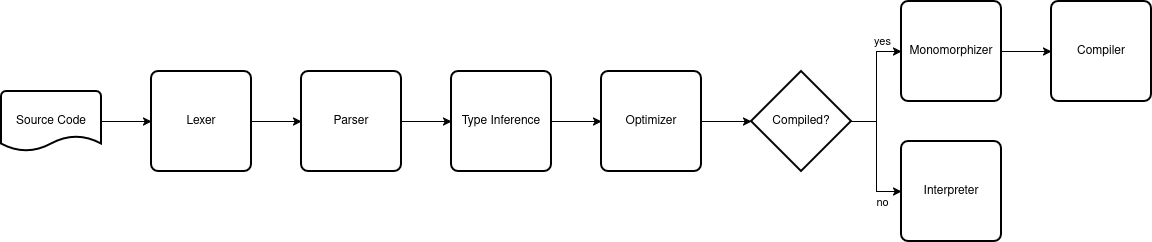
\includegraphics[width=\textwidth]{diagrams/DataFlow.png}
	\caption{Data Flow of the Implementation}
\end{figure}
The data from the file with the source code goes through the lexer,
parser, type inference and optimizer no matter what, and then depending
on if the program should be compiled it goes through the monomorphizer and
the compiler instead of the interpreter. This logic is done at the time of compilation
of the implementation instead of at runtime by the build script.

\subsection{The Lexer}
The lexer of Imp is a simple single-pass lexer, that computes
the tokens on-demand. This is done to avoid memory
allocations other than creating the syntax tree.
Its state consists of solely its
current position in the source text as well as the start
of the current token.

The tokens generated contain full information
about their location in the source code.

\subsubsection{Token Types}
The types of tokens that are returned by the lexer are:
\begin{itemize}
	\item The Keywords $let$ and $in$, $lambda$, $if$, $then$ and $else$,
	      $case$ and $of$, $or$, and $and$,
	\item the special characters $.$, $=$, $:$, $($ and $)$, $[$ and $]$
	\item the special sequences $->$ and $=>$,
	\item all operators for comparison and mathematical operations,
	      and the special operator $;$ which discards the first argument,
	\item Numbers, Booleans, Characters and Strings,
	\item Identifiers, which start with a letter and
	      then continue using alphanumeric characters or underscores,
	\item and Special Tokens for new lines and the end of the file
\end{itemize}

This means that all keywords are reserved and cannot be used
for the name of a variable.

\subsection{The Parser}
\importListing{code/expressions.tex}

The Parser consists of a pretty straight-forward implementation of the Pratt Parsing algorithm
for the expressions as shown in Listing \ref{listing:expressions} and a simple loop for statements.
In this implementation, the lookup table is represented by two functions,
$getNud$ and $getLed$.
The problem that there might not be an entry is solved by returning null
in that case.

Precedence for operators in $getLed$ is the following:
The most precedence of all operators is assigned to the $^$ operator for exponentiation,
followed by $*$ and $/$, which have equal precedence and finally $+$ and $-$ with equal
precedence as well. This is done to match precedence as known in mathematics.
Following these mathematic operators in precedence are the comparison operators
$<$, $<=$, $==$, $>=$ $>$, all with the same precedence.
The least precedence of all operators is assigned to $;$.

$getLed$ specifically has the special case that all token types that are present in $getNud$
can be the start of an argument given to the expression parsed before, since calls are
made just by juxtaposition. This special rule has the highest precedence of all expression types
so that the result of two functions can be combined using an operator without parentheses.

\subsection{Type Checking/Inference}
The Type Checker is mostly implemented close to how the Algorithm J as described
by Damas and Milner\autocite{damasPrincipalTypeschemesFunctional1982} works.
There is however a significant difference to the original type system:
There exists a special type Number(a), which represents either a Float or an Int
and therefore can be unified with both. When unified, the runtime representation
is then Number(Int) or Number(Float).

\importListing{code/unify.tex}

This Logic is contained in the unification function outlined
in listing \ref{listing:unify} on line 18-19. It takes advantage of the logic
on lines 3-12 which unifies a generic type variable with any type.

The constrained Number(a) is printed similarly to how Type Class
constraints are shown in Haskell, namely the type Number(a) is printed as
$Number\:a => \tau$.

The most significant change to the Algorithm J itself however
lies in the fact that in order to be able
to compute free, meaning independent, type variables for generalization
faster, levels as described in \autocite{EfficientInsightfulGeneralization2022} are
used. However, they are called depth in the code.
These levels are assigned to new type variables based on how many let statements and expressions
deep the algorithm is currently and are corrected if unified with a variable of lesser depth.
If a type variable contained in the type of a variable assigned via a let statement or expression
has a higher depth than at the start of parsing this let statement or expression, the type variable must be
independent since it can't depend on a type of something from outside, like an argument to a function, otherwise
it would have had a lesser depth.

\subsection{The Optimizer}
\importListing{code/optimizer.tex}

The Optimizer works slightly different depending on whether
the code is interpreted or compiled. In the case that it is interpreted
the optimizer also combines lambdas into larger objects,
while the compiler can't work with this combined representation.
However, in both cases a list of bound variables is gathered per function definition,
needed since all functions are closures in Imp.
The outline of the optimizer is shown in Listing \ref{listing:optimizer}.

All run functions of each step

\subsection{The Interpreter}
The Interpreter is a simple tree-walking Interpreter.
The most important optimization it employs is proper tail call elimination,
meaning it doesn't make another stack frame if a function call is the last
thing a function does, making recursion feasible through
tail recursion. This function doesn't need to be the function in whose body the
execution is currently in. This is done by having the evaluation of an expression return
the next part of the syntax tree to evaluate, which is then repeatedly evaluated in a loop until the final result
is reached, removing additional tail calls on the stack.

Additionally, based on the combined lambdas and calls from the optimizer, it can
essentially treat consecutive lambdas like defining a single, multi-argument
function, avoiding to build up a huge call stack, resulting in less allocations
and faster execution in most cases.

\subsection{The Monomorphizer}
The Monomorphizer is a step only needed for the compiler.
First it replaces all instances of free, non-bound type variables
with the type of Int. This is needed because for example the empty list
can have the type of $List\:a$ for any $a$, but the conversion to LLVM IR later on still needs a concrete
type to determine the correct representation.

Once this replacement is done, it essentially eliminates all polymorphism by duplicating
the value assigned to each $let$ for each type it takes on
in the code of the program. This can be done because
in the Hindley-Milner type system, every value
can only take on a finite number of types and is needed later on
because LLVM doesn't allow polymorphism.

The whole transformation is done by a simple pass over the syntax tree, gathering
all the types a value takes on in the body of each let expression,
or in the rest of the file, in case of a let statement or a type declaration,
getting the instantiation of the $\forall\vec{a}$ back by comparing the generic
with the specific type.
Once all instantiations are gathered, it copies the syntax tree of the definition once each.

This method is essentially the same as the programming language implementation MLTon uses.\autocite{Monomorphise}

\subsection{The Compiler}
The Compiler then converts this
monomorphic syntax tree into \Gls{llvm} \Gls{ir} using the C \Gls{api} of LLVM, which
makes the creation of LLVM IR possible from C instead of C++ through
Zigs automatically generated \Gls{ffi}. Zigs \Gls{ffi} allows it to call
C functions directly by automatically generating the correct bindings using the
headers.

Closures are represented in the \Gls{ir} as a struct consisting of two pointers:
The first being the function pointer, the second being a pointer to the heap
where all bound variables are stored.

The functions generated and pointed to in the closure
take two arguments each: Their actual argument
as declared by the source code, and the environment that had been stored
at the time of the closures creation.

Here, little is done to optimize the \Gls{ir} created apart
from recursive calls being done directly instead of through an indirect
call, as all other function calls are done in order to enable
the tail recursion optimization as it could not resolve the indirect function call
as a recursive call since it would be given via an argument and therefore
could theoretically be different.

Then clang is called on the \Gls{ir}, linking it with a very small library of built-in
functions with the highest optimization level of -O3. The tool therefore requires
clang to be present and on the PATH.

\section{Results}
Too see how programs in this language look, the following program, which
can be used to generate the fibonacci sequence,
will be explained.

\importListing{code/fibonacci.tex}

In this example, the fibonacci sequence is computed in the function
$fibonacciHelper$ through tail recursion. Because of that, that function
can be viewed as a loop which changes the variables $previous$, $current$ and
$n$ on each iteration. This change is done on line 6.

Throughout its execution, it also prints the current fibonacci number
computed using the two built-in functions $showInt$ and $print$.
$showInt$ is a function that converts an integer into a list of characters.

Several expressions are separated by a semicolon ($;$) which is an operator
in this language that simply discards the result on the left, meaning
the expression on the left is only there for its side-effects like printing.

The main function takes a dummy argument x, because in Imp, there are no
functions that take no argument. This function is then called
after all definitions have been executed.
On line 17 it then reads the number of elements requested,
which is then parsed. As this can fail, this returns a
value of type Option. The case expression then evaluates either line
18, if the parse failed, which just repeats the main function,
or it puts the result into the variable n which is then used in
lines 20-23. Finally on line 24, Void is returned, since Imp functions
also need to return exactly one value.

This example also demonstrates the power of Hindley-Milner type inference,
because no types did ever need to be annotated for the code to work,
but it is still garanteed that the whole program has no type errors.
The type given to fibonacciHelper is only there for clarity.

Other examples of Imp code can be found in the folder $examples$ in
the source code.

Additionally, to get a view of how the LLVM IR transformation works, here is
an example of the resulting IR of a simple function,
though cleaned up to remove clutter and add meaningful names.

\begin{minipage}{\linewidth}
	\begin{lstlisting}[
	% there are many more options of styling, see the official documentation, these are just the defaults I like
	frame=single, % make single-line frame around the verbatim
	framesep=2mm, % put some more spacing between the frame and text
	aboveskip=5mm, % put some more space above the box
	basicstyle={\linespread{0.9}\small\ttfamily}, % use typewriter (monospace) font
	caption={Add function in Imp}, % set the caption text
	captionpos=b, % put the caption at the bottom (b) or top (t) or both (bt)
    label={listing:addImp}, % label to be referenced via \ref{}
	numbers=left, % line numbers on the left
	numberstyle={\scriptsize\ttfamily\color{black!60}}, % the style for line numbers
	escapeinside={<@}{@>} % between those sequences are commands evaluated
]
<@\textcolor[HTML]{3010CF}{\textit{\textbf{\texttt{let}}}}@><@\textcolor[HTML]{000000}{\texttt{\ }}@><@\textcolor[HTML]{255CFF}{\texttt{add}}@><@\textcolor[HTML]{000000}{\texttt{:\ }}@><@\textcolor[HTML]{1F8F42}{\texttt{Int\ ->\ Int\ ->\ Int}}@><@\textcolor[HTML]{000000}{\texttt{\ }}@><@\textcolor[HTML]{1041FF}{\texttt{=}}@>
<@\textcolor[HTML]{000000}{\texttt{\ \ \ \ }}@><@\textcolor[HTML]{3010CF}{\textit{\textbf{\texttt{lambda}}}}@><@\textcolor[HTML]{000000}{\texttt{\ }}@><@\textcolor[HTML]{EA5110}{\textit{\texttt{x}}}@><@\textcolor[HTML]{1041FF}{\texttt{.}}@><@\textcolor[HTML]{000000}{\texttt{\ }}@><@\textcolor[HTML]{3010CF}{\textit{\textbf{\texttt{lambda}}}}@><@\textcolor[HTML]{000000}{\texttt{\ }}@><@\textcolor[HTML]{EA5110}{\textit{\texttt{y}}}@><@\textcolor[HTML]{1041FF}{\texttt{.}}@>
<@\textcolor[HTML]{000000}{\texttt{\ \ \ \ \ \ \ \ }}@><@\textcolor[HTML]{EA5110}{\textit{\texttt{x}}}@><@\textcolor[HTML]{000000}{\texttt{\ }}@><@\textcolor[HTML]{1041FF}{\texttt{+}}@><@\textcolor[HTML]{000000}{\texttt{\ }}@><@\textcolor[HTML]{EA5110}{\textit{\texttt{y}}}@>

\end{lstlisting}
	\begin{lstlisting}[
	% there are many more options of styling, see the official documentation, these are just the defaults I like
	frame=single, % make single-line frame around the verbatim
	framesep=2mm, % put some more spacing between the frame and text
	aboveskip=5mm, % put some more space above the box
	basicstyle={\linespread{0.9}\small\ttfamily}, % use typewriter (monospace) font
	caption={Add function compiled to LLVM IR}, % set the caption text
	captionpos=b, % put the caption at the bottom (b) or top (t) or both (bt)
    label={listing:addLLVM}, % label to be referenced via \ref{}
	numbers=left, % line numbers on the left
	numberstyle={\scriptsize\ttfamily\color{black!60}}, % the style for line numbers
	escapeinside={<@}{@>} % between those sequences are commands evaluated
]
<@\textcolor[HTML]{3010CF}{\textbf{\texttt{define}}}@><@\textcolor[HTML]{000000}{\texttt{\ }}@><@\textcolor[HTML]{FF1010}{\texttt{\{}}@><@\textcolor[HTML]{1F8F42}{\texttt{\ }}@><@\textcolor[HTML]{10909F}{\texttt{ptr}}@><@\textcolor[HTML]{1041FF}{\texttt{,}}@><@\textcolor[HTML]{1F8F42}{\texttt{\ }}@><@\textcolor[HTML]{10909F}{\texttt{ptr}}@><@\textcolor[HTML]{1F8F42}{\texttt{\ }}@><@\textcolor[HTML]{FF1010}{\texttt{\}}}@><@\textcolor[HTML]{000000}{\texttt{\ }}@><@\textcolor[HTML]{000000}{\texttt{@add}}@><@\textcolor[HTML]{FF1010}{\texttt{(}}@><@\textcolor[HTML]{10909F}{\texttt{i64}}@><@\textcolor[HTML]{EA5110}{\textit{\texttt{\ }}}@><@\textcolor[HTML]{000000}{\texttt{\%x}}@><@\textcolor[HTML]{1041FF}{\texttt{,}}@><@\textcolor[HTML]{000000}{\texttt{\ }}@><@\textcolor[HTML]{10909F}{\texttt{ptr}}@><@\textcolor[HTML]{EA5110}{\textit{\texttt{\ }}}@><@\textcolor[HTML]{000000}{\texttt{\%bound}}@><@\textcolor[HTML]{FF1010}{\texttt{)}}@><@\textcolor[HTML]{000000}{\texttt{\ }}@><@\textcolor[HTML]{FF1010}{\texttt{\{}}@>
<@\textcolor[HTML]{7777BB}{\texttt{entry:}}@>
<@\textcolor[HTML]{000000}{\texttt{\ \ }}@><@\textcolor[HTML]{000000}{\texttt{\%int\_ptr}}@><@\textcolor[HTML]{000000}{\texttt{\ }}@><@\textcolor[HTML]{1041FF}{\texttt{=}}@><@\textcolor[HTML]{000000}{\texttt{\ }}@><@\textcolor[HTML]{1010FF}{\texttt{getelementptr}}@><@\textcolor[HTML]{000000}{\texttt{\ }}@><@\textcolor[HTML]{FF1010}{\texttt{\{}}@><@\textcolor[HTML]{1F8F42}{\texttt{\ }}@><@\textcolor[HTML]{10909F}{\texttt{i64}}@><@\textcolor[HTML]{1F8F42}{\texttt{\ }}@><@\textcolor[HTML]{FF1010}{\texttt{\}}}@><@\textcolor[HTML]{1041FF}{\texttt{,}}@><@\textcolor[HTML]{000000}{\texttt{\ }}@><@\textcolor[HTML]{10909F}{\texttt{ptr}}@><@\textcolor[HTML]{000000}{\texttt{\ }}@><@\textcolor[HTML]{EA5110}{\textit{\texttt{null}}}@><@\textcolor[HTML]{1041FF}{\texttt{,}}@><@\textcolor[HTML]{000000}{\texttt{\ }}@><@\textcolor[HTML]{10909F}{\texttt{i32}}@><@\textcolor[HTML]{000000}{\texttt{\ }}@><@\textcolor[HTML]{EA5110}{\texttt{1}}@>
<@\textcolor[HTML]{000000}{\texttt{\ \ }}@><@\textcolor[HTML]{000000}{\texttt{\%sizeof\_int}}@><@\textcolor[HTML]{000000}{\texttt{\ }}@><@\textcolor[HTML]{1041FF}{\texttt{=}}@><@\textcolor[HTML]{000000}{\texttt{\ }}@><@\textcolor[HTML]{1010FF}{\texttt{ptrtoint}}@><@\textcolor[HTML]{000000}{\texttt{\ }}@><@\textcolor[HTML]{10909F}{\texttt{ptr}}@><@\textcolor[HTML]{000000}{\texttt{\ }}@><@\textcolor[HTML]{000000}{\texttt{\%int\_ptr}}@><@\textcolor[HTML]{000000}{\texttt{\ }}@><@\textcolor[HTML]{3010CF}{\textit{\textbf{\texttt{to}}}}@><@\textcolor[HTML]{000000}{\texttt{\ }}@><@\textcolor[HTML]{10909F}{\texttt{i64}}@>
<@\textcolor[HTML]{000000}{\texttt{\ \ }}@><@\textcolor[HTML]{000000}{\texttt{\%new\_bound}}@><@\textcolor[HTML]{000000}{\texttt{\ }}@><@\textcolor[HTML]{1041FF}{\texttt{=}}@><@\textcolor[HTML]{000000}{\texttt{\ }}@><@\textcolor[HTML]{1010FF}{\texttt{call}}@><@\textcolor[HTML]{000000}{\texttt{\ }}@><@\textcolor[HTML]{10909F}{\texttt{ptr}}@><@\textcolor[HTML]{000000}{\texttt{\ }}@><@\textcolor[HTML]{000000}{\texttt{@GC\_malloc}}@><@\textcolor[HTML]{FF1010}{\texttt{(}}@><@\textcolor[HTML]{10909F}{\texttt{i64}}@><@\textcolor[HTML]{EA5110}{\textit{\texttt{\ }}}@><@\textcolor[HTML]{000000}{\texttt{\%sizeof\_int}}@><@\textcolor[HTML]{FF1010}{\texttt{)}}@>
<@\textcolor[HTML]{000000}{\texttt{\ \ }}@><@\textcolor[HTML]{000000}{\texttt{\%x\_location}}@><@\textcolor[HTML]{000000}{\texttt{\ }}@><@\textcolor[HTML]{1041FF}{\texttt{=}}@><@\textcolor[HTML]{000000}{\texttt{\ }}@><@\textcolor[HTML]{1010FF}{\texttt{getelementptr}}@><@\textcolor[HTML]{000000}{\texttt{\ }}@><@\textcolor[HTML]{FF1010}{\texttt{\{}}@><@\textcolor[HTML]{1F8F42}{\texttt{\ }}@><@\textcolor[HTML]{10909F}{\texttt{i64}}@><@\textcolor[HTML]{1F8F42}{\texttt{\ }}@><@\textcolor[HTML]{FF1010}{\texttt{\}}}@><@\textcolor[HTML]{1041FF}{\texttt{,}}@><@\textcolor[HTML]{000000}{\texttt{\ }}@><@\textcolor[HTML]{10909F}{\texttt{ptr}}@><@\textcolor[HTML]{000000}{\texttt{\ }}@><@\textcolor[HTML]{000000}{\texttt{\%new\_bound}}@><@\textcolor[HTML]{1041FF}{\texttt{,}}@><@\textcolor[HTML]{000000}{\texttt{\ }}@><@\textcolor[HTML]{10909F}{\texttt{i32}}@><@\textcolor[HTML]{000000}{\texttt{\ }}@><@\textcolor[HTML]{EA5110}{\texttt{0}}@><@\textcolor[HTML]{1041FF}{\texttt{,}}@><@\textcolor[HTML]{000000}{\texttt{\ }}@><@\textcolor[HTML]{10909F}{\texttt{i32}}@><@\textcolor[HTML]{000000}{\texttt{\ }}@><@\textcolor[HTML]{EA5110}{\texttt{0}}@>
<@\textcolor[HTML]{000000}{\texttt{\ \ }}@><@\textcolor[HTML]{1010FF}{\texttt{store}}@><@\textcolor[HTML]{000000}{\texttt{\ }}@><@\textcolor[HTML]{10909F}{\texttt{i64}}@><@\textcolor[HTML]{000000}{\texttt{\ }}@><@\textcolor[HTML]{000000}{\texttt{\%x}}@><@\textcolor[HTML]{1041FF}{\texttt{,}}@><@\textcolor[HTML]{000000}{\texttt{\ }}@><@\textcolor[HTML]{10909F}{\texttt{ptr}}@><@\textcolor[HTML]{000000}{\texttt{\ }}@><@\textcolor[HTML]{000000}{\texttt{\%x\_location}}@>
<@\textcolor[HTML]{000000}{\texttt{\ \ }}@><@\textcolor[HTML]{000000}{\texttt{\%add\_const\_closure}}@><@\textcolor[HTML]{000000}{\texttt{\ }}@><@\textcolor[HTML]{1041FF}{\texttt{=}}@><@\textcolor[HTML]{000000}{\texttt{\ }}@><@\textcolor[HTML]{1010FF}{\texttt{insertvalue}}@><@\textcolor[HTML]{000000}{\texttt{\ }}@><@\textcolor[HTML]{FF1010}{\texttt{\{}}@><@\textcolor[HTML]{1F8F42}{\texttt{\ }}@><@\textcolor[HTML]{10909F}{\texttt{ptr}}@><@\textcolor[HTML]{1041FF}{\texttt{,}}@><@\textcolor[HTML]{1F8F42}{\texttt{\ }}@><@\textcolor[HTML]{10909F}{\texttt{ptr}}@><@\textcolor[HTML]{1F8F42}{\texttt{\ }}@><@\textcolor[HTML]{FF1010}{\texttt{\}}}@><@\textcolor[HTML]{000000}{\texttt{\ }}@><@\textcolor[HTML]{FF1010}{\texttt{\{}}@><@\textcolor[HTML]{724BFF}{\textit{\texttt{\ }}}@><@\textcolor[HTML]{10909F}{\texttt{ptr}}@><@\textcolor[HTML]{724BFF}{\textit{\texttt{\ }}}@><@\textcolor[HTML]{000000}{\texttt{@add\_const}}@><@\textcolor[HTML]{1041FF}{\texttt{,}}@><@\textcolor[HTML]{724BFF}{\textit{\texttt{\ }}}@><@\textcolor[HTML]{10909F}{\texttt{ptr}}@><@\textcolor[HTML]{724BFF}{\textit{\texttt{\ }}}@><@\textcolor[HTML]{EA5110}{\textit{\texttt{undef}}}@><@\textcolor[HTML]{724BFF}{\textit{\texttt{\ }}}@><@\textcolor[HTML]{FF1010}{\texttt{\}}}@><@\textcolor[HTML]{1041FF}{\texttt{,}}@><@\textcolor[HTML]{000000}{\texttt{\ }}@><@\textcolor[HTML]{10909F}{\texttt{ptr}}@><@\textcolor[HTML]{000000}{\texttt{\ }}@><@\textcolor[HTML]{000000}{\texttt{\%new\_bound}}@><@\textcolor[HTML]{1041FF}{\texttt{,}}@><@\textcolor[HTML]{000000}{\texttt{\ }}@><@\textcolor[HTML]{EA5110}{\texttt{1}}@>
<@\textcolor[HTML]{000000}{\texttt{\ \ }}@><@\textcolor[HTML]{1010FF}{\textit{\texttt{ret}}}@><@\textcolor[HTML]{000000}{\texttt{\ }}@><@\textcolor[HTML]{FF1010}{\texttt{\{}}@><@\textcolor[HTML]{1F8F42}{\texttt{\ }}@><@\textcolor[HTML]{10909F}{\texttt{ptr}}@><@\textcolor[HTML]{1041FF}{\texttt{,}}@><@\textcolor[HTML]{1F8F42}{\texttt{\ }}@><@\textcolor[HTML]{10909F}{\texttt{ptr}}@><@\textcolor[HTML]{1F8F42}{\texttt{\ }}@><@\textcolor[HTML]{FF1010}{\texttt{\}}}@><@\textcolor[HTML]{000000}{\texttt{\ }}@><@\textcolor[HTML]{000000}{\texttt{\%add\_const\_closure}}@>
<@\textcolor[HTML]{FF1010}{\texttt{\}}}@>

<@\textcolor[HTML]{3010CF}{\textbf{\texttt{define}}}@><@\textcolor[HTML]{000000}{\texttt{\ }}@><@\textcolor[HTML]{10909F}{\texttt{i64}}@><@\textcolor[HTML]{000000}{\texttt{\ }}@><@\textcolor[HTML]{000000}{\texttt{@add\_const}}@><@\textcolor[HTML]{FF1010}{\texttt{(}}@><@\textcolor[HTML]{10909F}{\texttt{i64}}@><@\textcolor[HTML]{EA5110}{\textit{\texttt{\ }}}@><@\textcolor[HTML]{000000}{\texttt{\%y}}@><@\textcolor[HTML]{1041FF}{\texttt{,}}@><@\textcolor[HTML]{000000}{\texttt{\ }}@><@\textcolor[HTML]{10909F}{\texttt{ptr}}@><@\textcolor[HTML]{EA5110}{\textit{\texttt{\ }}}@><@\textcolor[HTML]{000000}{\texttt{\%bound}}@><@\textcolor[HTML]{FF1010}{\texttt{)}}@><@\textcolor[HTML]{000000}{\texttt{\ }}@><@\textcolor[HTML]{FF1010}{\texttt{\{}}@>
<@\textcolor[HTML]{7777BB}{\texttt{entry:}}@>
<@\textcolor[HTML]{000000}{\texttt{\ \ }}@><@\textcolor[HTML]{000000}{\texttt{\%x\_location}}@><@\textcolor[HTML]{000000}{\texttt{\ }}@><@\textcolor[HTML]{1041FF}{\texttt{=}}@><@\textcolor[HTML]{000000}{\texttt{\ }}@><@\textcolor[HTML]{1010FF}{\texttt{getelementptr}}@><@\textcolor[HTML]{000000}{\texttt{\ }}@><@\textcolor[HTML]{FF1010}{\texttt{\{}}@><@\textcolor[HTML]{1F8F42}{\texttt{\ }}@><@\textcolor[HTML]{10909F}{\texttt{i64}}@><@\textcolor[HTML]{1F8F42}{\texttt{\ }}@><@\textcolor[HTML]{FF1010}{\texttt{\}}}@><@\textcolor[HTML]{1041FF}{\texttt{,}}@><@\textcolor[HTML]{000000}{\texttt{\ }}@><@\textcolor[HTML]{10909F}{\texttt{ptr}}@><@\textcolor[HTML]{000000}{\texttt{\ }}@><@\textcolor[HTML]{000000}{\texttt{\%bound}}@><@\textcolor[HTML]{1041FF}{\texttt{,}}@><@\textcolor[HTML]{000000}{\texttt{\ }}@><@\textcolor[HTML]{10909F}{\texttt{i32}}@><@\textcolor[HTML]{000000}{\texttt{\ }}@><@\textcolor[HTML]{EA5110}{\texttt{0}}@><@\textcolor[HTML]{1041FF}{\texttt{,}}@><@\textcolor[HTML]{000000}{\texttt{\ }}@><@\textcolor[HTML]{10909F}{\texttt{i32}}@><@\textcolor[HTML]{000000}{\texttt{\ }}@><@\textcolor[HTML]{EA5110}{\texttt{0}}@>
<@\textcolor[HTML]{000000}{\texttt{\ \ }}@><@\textcolor[HTML]{000000}{\texttt{\%x}}@><@\textcolor[HTML]{000000}{\texttt{\ }}@><@\textcolor[HTML]{1041FF}{\texttt{=}}@><@\textcolor[HTML]{000000}{\texttt{\ }}@><@\textcolor[HTML]{1010FF}{\texttt{load}}@><@\textcolor[HTML]{000000}{\texttt{\ }}@><@\textcolor[HTML]{10909F}{\texttt{i64}}@><@\textcolor[HTML]{1041FF}{\texttt{,}}@><@\textcolor[HTML]{000000}{\texttt{\ }}@><@\textcolor[HTML]{10909F}{\texttt{ptr}}@><@\textcolor[HTML]{000000}{\texttt{\ }}@><@\textcolor[HTML]{000000}{\texttt{\%x\_location}}@>
<@\textcolor[HTML]{000000}{\texttt{\ \ }}@><@\textcolor[HTML]{000000}{\texttt{\%result}}@><@\textcolor[HTML]{000000}{\texttt{\ }}@><@\textcolor[HTML]{1041FF}{\texttt{=}}@><@\textcolor[HTML]{000000}{\texttt{\ }}@><@\textcolor[HTML]{1010FF}{\texttt{add}}@><@\textcolor[HTML]{000000}{\texttt{\ }}@><@\textcolor[HTML]{10909F}{\texttt{i64}}@><@\textcolor[HTML]{000000}{\texttt{\ }}@><@\textcolor[HTML]{000000}{\texttt{\%x}}@><@\textcolor[HTML]{1041FF}{\texttt{,}}@><@\textcolor[HTML]{000000}{\texttt{\ }}@><@\textcolor[HTML]{000000}{\texttt{\%y}}@>
<@\textcolor[HTML]{000000}{\texttt{\ \ }}@><@\textcolor[HTML]{1010FF}{\textit{\texttt{ret}}}@><@\textcolor[HTML]{000000}{\texttt{\ }}@><@\textcolor[HTML]{10909F}{\texttt{i64}}@><@\textcolor[HTML]{000000}{\texttt{\ }}@><@\textcolor[HTML]{000000}{\texttt{\%result}}@>
<@\textcolor[HTML]{FF1010}{\texttt{\}}}@>

\end{lstlisting}

\end{minipage}

The first lambda defined on line 2 of Listing \ref{listing:addImp} got transformed
into the function $@add$ of Listing \ref{listing:addLLVM}.
As the second lambda binds the value of $x$, $@add$ allocates
enough memory to store it on lines 3-5, then gets the exact location on line 6, which
is done since there might be more than one bound variable, but in this case is redundant.
Line 7 then stores $x$ while line 8 creates the closure by inserting the pointer to the bound
variable in a struct.
Finally on line 9, the closure is returned.

The function $@add\_const$ then accesses this bound variable, again first getting the
location on the redundant line 14, then loads the actual value of $x$ on line 15
and finally computes the result on line 16 which is returned on line 17.

To compare the performance of the two implementations with a real-world language,
a small benchmark was run using a tool called hyperfine\autocite{peterHyperfine2023}.
Both the Imp and the Python implementation compute and print the mandelbrot set.
For the compiler, only the compiled program was benchmarked, and not
the time it takes to compile it. The version of LLVM used was 20.1.8.
The Python implementation is to compare the Imp language to a language used in
real-world usecases. It was run using Python 3.12.1.
All the files being benchmarked can be found in the folder \path{benchmark}.

\begin{table}[H]
	\centering
	\begin{tabular}{|l|l|l|l|}
		\hline
		Language             & Mean [ms]    & Min [ms] & Max [ms] \\ \hline
		Imp with Compiler    & 9.7 ± 2.7    & 5.3      & 16.9     \\ \hline
		Imp with Interpreter & 390.1 ± 16.9 & 362.2    & 421.2    \\ \hline
		Python               & 57.9 ± 8.0   & 40.1     & 73.7     \\ \hline
	\end{tabular}
\end{table}

As can be seen in this table, the language Imp is slower than Python in this case if interpreted,
but the compiler brought an improvement of approxmately 40x over the interpreter, while Python
takes almost 6 times the time that the compiled program takes.

\section{Discussion}
As seen in the example given, the language
can be used for mathematical computation.
Both the interpreter and compiler are also relatively fast and
(with a minor caveat) memory-safe. The feasability of this method of
compilation was shown by the benchmark.

However, there are also several
shortcomings that will be mentioned here.

\subsection{Shortcomings}\label{shortcomings}
The language Imp is a functioning prototype, but there are several
aspects which would need to be treated in order for this language
to be useful for any practical purposes.

\subsubsection{Input/output}
Input/output is an essential part of any programming language.
The language Imp is no exception to this, having the two functions
$print$ and $read$ which print to standard output and read from
standard input respectively. However, there is currently no way
to read from or write to files, which is essential for a program
to store information for later usages of it or to load and/or output larger
amounts of information.

To enable this feature, a type for Files or Buffers would have to be
introduced for fast, type-safe interaction.

\subsubsection{Library System}
In Imp, it is impossible to import other files from a program.
This would be essential however for the development of libraries.
To enable imports and therefore libraries, a topological sorting
algorithm could be used, since the order of definitions does
matter in this language and circular references can't exist anyway.

This would enable a much more practical implementation of the standard
library as well, since e.g. functions that operate on functions could be used
in almost all other parts of the library.

\subsubsection{FFI}
At the moment, Imp cannot access system libraries or libraries
written in other languages at all, meaning GUIs or even most TUIs
(terminal user interfaces) are impossible to create,
since you couldn't use libraries like QT.

This could be mitigated by a large set of built-in functions based
on which a standard library could be built, or more simply, though
less securely, using an FFI (foreign function interface).

Using a foreign function interface, one could declare functions that
exist in another language (most likely C), and their types and then use
those functions. This would lead to other challenges however, since
there exists no equivalent to many of the types in C.
The types would however need to match up exactly,
putting a huge burden on both the programmer writing the declarations
as there should be no type errors, otherwise the whole type system
would be for nothing, and the compiler, as it would no longer
be free to represent its objects however it wants.
LLVM does also not garantee correct FFI, even if the types
seem to match up.

\subsubsection{OS Compatibility}
As the Compiler of this language depends on both
LLVM and Boehm \Gls{gc}, it can only be used on Operating Systems
that support both of these. However, Linux, MacOS and Windows
are all supported by them both.

Windows has however the problem of there not being
a prebuilt package for LLVM which includes the headers as well
as the libraries to be linked and doesn't depend on MSVC and its
implementation of the C/C++ standard libraries.

However, as Zig doesn't compile parts of the code it sees are not needed,
LLVM not being available doesn't prevent compilation and execution of the interpreter.
When building with \texttt{zig build}, it automatically decides whether to use
the compiler based on the operating system.

\subsection{Room for improvement}
There are many parts of both the compiler and the
interpreter, which could be improved significantly
for enhanced speed and better memory consumption.

\subsubsection{Garbage Collector}
Though both the compiler and the interpreter produce
garbage collected programs, the compiler uses the
conservative Boehm-Demers-Weiser \Gls{gc} \autocite{GarbageCollector},
which is unaware of any of the types of Imp and therefore
has to assume that anything that could be a pointer,
is in fact a pointer. It should therefore be replaced with
precise \Gls{gc} to prevent leaks caused by values randomly looking
like pointers.
Meanwhile, the interpreter uses a very basic mark-and-sweep
\Gls{gc}. However this could very easily be improved
by using methods like Generational Garbage Collection, where
young objects are checked more often than older ones, which are more
likely to live for the entirety of the program.

\subsubsection{Defunctionalization}
Furthermore, another possible optimization done by almost all
functional programming languages nowadays is some form of
defunctionalization, which is a process which tries
to eliminate functions as arguments, replacing them with
an object that is given as an argument which denotes which
function it represents.

One new interesting approach that seems to be promising
is the technique of lambda set specialization
\autocite{brandonBetterDefunctionalizationLambda2023a}, which
could be applied to this language relatively easily,
since it assumes a Hindley-Milner style type inference
as well.

\section{Conclusions}
In conclusion, almost all the goals were met.
The language is now fully functional and able to be tested by anyone.
There are a few aspects that would need to be improved for it to be
useful for anything practical as explained in section \ref{shortcomings},
but it is already a useable language.

However, the goal for the language to be cross-platform has not really been met,
as while the Interpreter is theoretically working on all systems supported by zig
that have a file system and a standard in- and output, the compiler only works on
Linux at the moment.

The language created could now be used as a starting point for a more useful and
feature-rich language.

\newpage
\printbibliography

\newpage
\lstlistoflistings
\listoffigures

\newpage
\printglossaries

\appendix

\section{Source Code}
The source code for the compiler and interpreter can be found on
\href{https://github.com/enmiligi/matura-project}{GitHub}.
The tree-sitter parser can be found \href{https://github.com/enmiligi/tree-sitter-imp}{here}
and the extension for Zed enabling syntax highlighting is located \href{https://github.com/enmiligi/zed-imp}{here}.

\end{document}
